\documentclass{standalone}
\usepackage{amssymb,amsmath}
\usepackage{tikz}
\usetikzlibrary{automata,positioning}
\begin{document}
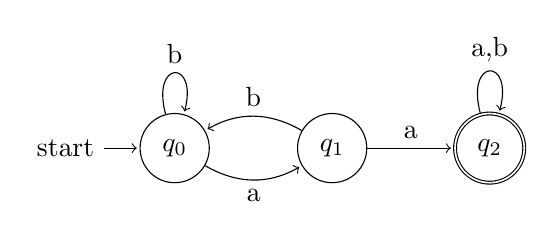
\begin{tikzpicture}[shorten >=1pt,node distance=2cm,on grid,auto] 
 \node[state,initial] (s_0) {$q_0$};
 \node[state] (s_a)[right=of s_0] {$q_1$};
 \node[state,accepting] (s_ab)[right=of s_a] {$q_2$};
 \path[->] 
 (s_0) edge [loop above] node {b} (s_0)
 (s_0) edge [bend right,below] node {a} (s_a)
 (s_a) edge [bend right,above] node {b} (s_0)
 (s_a) edge [above] node {a} (s_ab)
 (s_ab) edge [loop above] node {a,b} (s_ab);
\end{tikzpicture} 
 \end{document}